%
%  Mikroprozessor Praktikum Protokolle
%
%  Sebastian Raitza, Nico von Geyso 2010
%
\documentclass[11pt,german]{scrartcl}

% See geometry.pdf to learn the layout options.
\usepackage{geometry}
\geometry{a4paper}

% To begin paragraphs with an empty line
\usepackage[parfill]{parskip}

% Use utf-8 encoding for foreign characters
\usepackage[utf8]{inputenc}
\usepackage[T1]{fontenc}

% Setup for fullpage use
\usepackage{fullpage}

% More symbols
\usepackage{amsmath}
\usepackage{amssymb}
%\usepackage{latexsym}

% Surround parts of graphics with box
\usepackage{boxedminipage}

% Package for including code in the document
\usepackage{listings}
\usepackage{color}
\usepackage{moreverb}
\usepackage{courier}


% This is now the recommended way for checking for PDFLaTeX:
\usepackage{ifpdf}

\ifpdf
\usepackage[pdftex]{graphicx}
\else
\usepackage{graphicx}
\fi

\ifpdf
\DeclareGraphicsExtensions{.pdf, .jpg, .tif}
\else
\DeclareGraphicsExtensions{.eps, .jpg}
\fi

% Create hyperlinks
\usepackage{hyperref}
\hypersetup{
    colorlinks=false,       % false: boxed links; true: colored links
    linkcolor=red,          % color of internal links
    citecolor=green,        % color of links to bibliography
    filecolor=magenta,      % color of file links
    urlcolor=cyan           % color of external links
}

\title{Mikroprozessor Praktikum\\Protokolle 1-15}
\author{Sebastian Raitza, Nico von Geyso}

% Activate to display a given date or no date
%\date{}

%%%%%%%%%%%%%%%%%%%%%%%%%%%%%%%%%%%%%%%%%%%%%%%%%%%%%%%%%%%%%%%%%%

\renewcommand{\labelenumi}{\alph{enumi})}
\renewcommand{\labelenumii}{$\bullet$}

% define a macro ausgabe which takes as argument
% your ausgabe.txt file’s name
\newcommand{\ausgabe}[1] {\hrule\small\verbatiminput{#1}\normalsize\hrule}

\definecolor{light-gray}{gray}{0.95}

\lstset{
  language=C,               % choose the language of the code
  basicstyle=\ttfamily\scriptsize,   % size of fonts used for the code
  numbers=left,             % where to put the line-numbers
  numberstyle=\scriptsize,        % size of fonts for used line-numbers
  stepnumber=1,             % step between line-numbers
  numbersep=5pt,            % how far the line-numbers are from the code
  backgroundcolor=\color{white},  % background color, add \usepackage{color}
  showspaces=false,         % show spaces adding particular underscores
  showstringspaces=false,   % underline spaces within strings
  showtabs=false,           % show tabs within strings adding particular underscores
  frame=single,             % adds a frame around the code
  tabsize=4,                % sets default tabsize to 2 spaces
  captionpos=b,             % sets the caption-position to bottom
  breaklines=true,          % sets automatic line breaking
  breakatwhitespace=false,  % sets if automatic breaks should only happen at whitespace
  escapeinside={\%*}{*)},   % if you want to add a comment within your code
  frameround=tttt,
  extendedchars=true,
  literate=%
    {Ö}{{\"O}}1
    {Ä}{{\"A}}1
    {Ü}{{\"U}}1
    {ß}{{\ss}}2
    {ü}{{\"u}}1
    {ä}{{\"a}}1
    {ö}{{\"o}}1
    {°}{{}}0
}

\begin{document}

\maketitle

\section{Modulbeschreibung des Mikroprozessor-Praktikum}
Die überwältigende Mehrheit zukünftiger Computersysteme wird durch miteinander kommunizierende, eingebettete Systeme geprägt sein.
Diese finden sich in Maschinensteuerungen, Haushaltsgeräten, Kraftfahrzeugen, Flugzeugen, intelligenten Gebäuden etc. und
werden zukünftig immer mehr in Netze wie dem Internet eingebunden sein.
Das Praktikum wird auf die Architektur eingebetteter Systeme eingehen und die Unterschiede zu traditionellen PC-Architekturen
(z.B. Echtzeitfähigkeit, Interaktion mit der Umgebung) anhand praktischer Beispiele aufzeigen.
Das Praktikum basiert auf einem MSP430 Mikrocontrollersystem.
Schwerpunkte des in einzelne Versuche gegliederten Praktikums sind:
\begin{itemize}
    \item Registerstrukturen
    \item Speicherorganisation
    \item hardwarenahe Assembler- und Hochsprachenprogrammierung
    \item I/O-System- und Timer-Programmierung
    \item Interrupt-System
    \item Watchdog-Logik
    \item Analogschnittstellen
    \item Bussystemanbindung von Komponenten
    \item Kommunikation (seriell, CAN-Bus, Ethernet, Funk und USB)
    \item Ansteuerung von Modellen und Nutzung unterschiedlichster Sensorik.
\end{itemize}


\section{Entwicklungsboard MSB430H}
Auf dem zum entwickelten Board handelt es sich um das Entwicklungsboard MSB430H.
Der hier verwendete Mikrocontroller ist ein MSP430F1612 von Texas Instrument.
Dieser verfügt neben einem universellen Clock-System unter anderem über 55 kByte Flash, 5kByte Ram, USART und einem Watchdog.
Das Board ist zusätzlich mit einem 868MHz Transciever (CC1100),
sowie einem Luftfeuchtigkeits- und Temperatursensor (SHT11), einem 3D-Beschleunigungssensor (MMA7260Q)
und einer SD-Karte ausgestattet.

%%%%%%%%%%%%%%%%%%%%%%%%%%%%%%%%%%%%%%%%%%%%%%%%%%%%%%%%%%%%%%%%%%

\clearpage
\section*
{\href{http://cst.mi.fu-berlin.de/intern/19606-P-MPP/Aufgaben/040100.html}
{I/O Portleitungen}}

Ein Kennzeichen von Mikrocontrollern sind seine I/O-Portleitungen.
Auch bekannt unter dem Namen \textit{General Purpose Input/Output}.
Diese Pins können als Eingang um digitale Signale zu lesen fungieren
oder als Ausgang um andere Geräte zu kontrollieren oder mit ihnen zu kommunizieren.

Die Konfiguration dieser kann mittels Software programmiert werden
und überlässt so dem Entwickler große Freiheiten.
Bei manchen Mikrocontrollern können einige I/O-Ports desweiteren als Interruptquellen definiert werden.

Meist werden die I/O-Pins in unterschiedliche Ports gruppiert.
Ein Port hat meistens acht I/O-Pins.

Der von uns verwendete MSP430F1612 verfügt über sechs I/O-Ports mit jeweils acht Bit Breite.

\subsection
{\href{http://cst.mi.fu-berlin.de/intern/19606-P-MPP/Aufgaben/040101.html}
{Aufgabe 1: Portleitung als Output}}

Jeder Pin kann über die 8-Bit Register PxDIR, PxOUT und PxIN konfiguriert beziehungsweise ausgelesen werden.
X ist dabei ein Wert zwischen 0 und 5 – stehend für den jeweiligen Port.

Mittels dem i-ten Bit des PxDIR-Registers wird der $i$-te Pin des Ports $x$ als Eingang oder Ausgang konfiguriert.
Je nachdem kann im PxIN-Register der Wert gelesen bzw. im PxOUT-Register geschrieben werden.

Die Pins selber können nur zwei Zustände annehmen: HIGH (logisch Eins) und LOW (logisch Null).
\subsubsection*{Erläuterung von Befehlen}
\lstinputlisting[linerange=29-41,firstnumber=29,caption=aufgabe01.c]
{../MPP_WS1011/aufgaben/aufgabe01.c}

\subsubsection*{Ampelschaltung}

Um eine Ampelschaltung zu realisieren wird in festeinprogrammierten Zeitabständen die jeweilige LED-Kombination eingeschaltet.
\lstinputlisting[linerange=46-70,firstnumber=46,caption=aufgabe01.c]
{../MPP_WS1011/aufgaben/aufgabe01.c}

\subsection*{Aufgabe 2: Portleitung als Input}

\subsubsection*{Erklärung der Befehlszeilen}
\lstinputlisting[linerange=16-29,firstnumber=16,caption=aufgabe02.c]
{../MPP_WS1011/aufgaben/aufgabe02.c}

\subsubsection*{Tastenprogramm}
\lstinputlisting[linerange=43-70,firstnumber=43,caption=aufgabe02.c]
{../MPP_WS1011/aufgaben/aufgabe02.c}

\subsection*{
\href{http://cst.mi.fu-berlin.de/intern/19606-P-MPP/Aufgaben/040103.html}
{Aufgabe 3: Ampelsteuerung}}

\lstinputlisting[linerange=17-83,firstnumber=17,caption=aufgabe03.c]
{../MPP_WS1011/aufgaben/aufgabe03.c}


\subsection
{\href{http://cst.mi.fu-berlin.de/intern/19606-P-MPP/Aufgaben/040104.html}
{Aufgabe 4: Tastaturabfrage}}
Je nachdem welche Taste gedrückt wird der interne Zähle in- bzw. dekrementiert oder zurückgesetzt. 
Für die binäre Darstellung wird mittels einfacher booleschen Und-Operation und Schiebeoperation das jeweilige Bit ermittelt und dann die dazugehörige LED umgeschaltet.
\lstinputlisting[linerange=17-53,firstnumber=17,caption=aufgabe04.c]
{../MPP_WS1011/aufgaben/aufgabe04.c}




%%%%%%%%%%%%%%%%%%%%%%%%%%%%%%%%%%%%%%%%%%%%%%%%%%%%%%%%%%%%%%%%%%

\clearpage
\section*
{\href{http://cst.mi.fu-berlin.de/intern/19606-P-MPP/Aufgaben/040200.html}
{Clock System}}

\subsection*
{\href{http://cst.mi.fu-berlin.de/intern/19606-P-MPP/Aufgaben/040201.html}
{Aufgabe 5: Frequenzmessung der Taktquellen}}

\subsubsection*{Vorbereitung}
\begin{lstlisting}
void Aufgabe5() {
    P5SEL |= BIT4;    // P5 MCLK
}
\end{lstlisting}

\subsubsection*{Messwerte}
\paragraph{LFXT1CL} \texttt{(SELM = 11b)}
\begin{description}
    \item [LF-Mode] \texttt{(XTS = 0)}
        \begin{enumerate}
            \item minimal: 12,29kHz, DIVM=11b
            \item maximal: 32,769, DIVM=00
        \end{enumerate}

    \item [HF-Mode] \texttt{(XTS = 1)}
        \begin{enumerate}
            \item minimal: 636,5kHz, DIVM=11b
            \item maximal: 1,695 MHz, DIVM=00
        \end{enumerate}
\end{description}

\paragraph{XT2CL} \texttt{(SELM = 11b, XT2OFF=0)}
\begin{enumerate}
    \item minimal: 635 KHz, DIVM=11b
    \item maximal: 1,695 MHz, DIVM=00
\end{enumerate}

\paragraph{DCOCLK} \texttt{(SELM = 00b)}
\begin{enumerate}
    \item minimal: 393,2 kHz, DCO=000b, RSEL=000b, DIVM=11b, MOD = 00000b
    \item normal: 7,36 mHz, DCO=011b, RSEL=100b, DIVM=00b, MOD = 11101b
    \item maximal: 11,59Mhz, DCO=111b, RSEL=111b, DIVM=00b, MOD hat keinen Effekt
\end{enumerate}

\paragraph{Erläutern Sie, wie der externe Widerstand für den DCOCLK-Taktgenerator nutzbar gemacht wird?}
Durch setzten des DCOR-Bits im BCSCTL2-Bit-Feld kann der externe Widerstand nutzbar gemacht werden.

\paragraph{Welchen Einfluss hat der Widerstand auf den DCOCLK-Taktgenerator?}
Der Widerstand verringert den Einfluss der Temperatur auf die Zuverlässigkeit des Taktgenerators. RC-Glied wieder niederohmiger und somit werden die Flanken deutlicher, da der Kondensator sich wieder schnell aufladen kann.


\subsection
{\href{http://cst.mi.fu-berlin.de/intern/19606-P-MPP/Aufgaben/040202.html}
{Aufgabe 6: Stromverbrauch und Taktfrequenz}}

Folgende Tabelle zeigt die Abhängigkeit des Stromverbrauchs von der Taktfrequenz. Der DCO\-CLK-Taktgenerator wurde durch manuelle Modifikation der DCOCTL, BCSCTL1 und BCSCTL2 Register im Debug-Modus des Code Composers auf Frequenzen im Bereich von 100kHz bis 10MHz eingestellt. Anschließend wurde jeweils der Stromverbrauch des Controllers im RUN-Modus am in Reihe geschalteten Digitalmultimeter gemessen. Die Tabelle enthält alle Messwerte mit den entsprechenden Bit-Settings der Clock-Register.

\begin{center}
\begin{tabular}{|r|c|c|c|c|c|}\hline
Frequenz in kHz	&	Strom in mA	&	RSEL	&	DCO	&	MOD	&	DIVM \\\hline

99,7	&	0,53	&	0	&	0	&	0	&	3 \\\hline
138,4	&	0,57	&	1	&	0	&	0	&	3 \\\hline
196,6	&	0,62	&	2	&	0	&	0	&	3 \\\hline
290,6	&	0,71	&	3	&	0	&	0	&	3 \\\hline
393,7	&	0,81	&	4	&	0	&	0	&	3 \\\hline
505,3	&	0,91	&	5	&	0	&	0	&	3 \\\hline
589,3	&	0,99	&	6	&	0	&	0	&	3 \\\hline
666,1	&	1,06	&	7	&	0	&	0	&	3 \\\hline
986,3	&	1,34	&	7	&	4	&	0	&	3 \\\hline
1.458,0	&	1,75	&	7	&	7	&	0	&	3 \\\hline
1.971,0	&	1,87	&	7	&	4	&	0	&	2 \\\hline
2.916,0	&	2,53	&	7	&	7	&	0	&	2 \\\hline
3.940,0	&	2,91	&	7	&	4	&	0	&	1 \\\hline
4.096,0	&	3,02	&	7	&	4	&	11	&	1 \\\hline
5.827,0	&	4,05	&	7	&	7	&	0	&	1 \\\hline
7.368,0	&	4,67	&	5	&	5	&	29	&	0 \\\hline
7.870,0	&	4,94	&	7	&	4	&	0	&	0 \\\hline
11.612,0	&	6,88	&	7	&	7	&	0	&	0 \\\hline

\end{tabular}
\end{center}

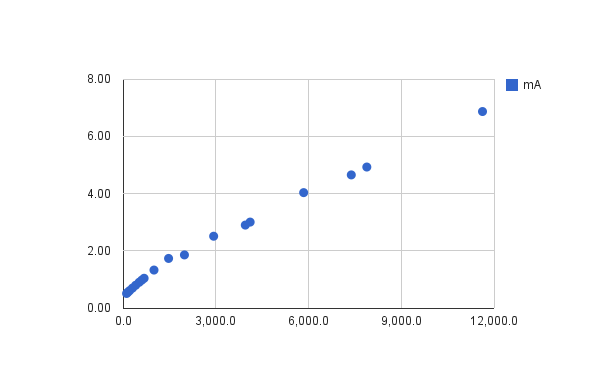
\includegraphics[width=\textwidth]{aufgaben/06/chart_2.png}

Das Diagramm zeigt den Stromverbrauch (vertikal) im Verhältnis zur Taktfrequenz (horizontal) der MCLK an Hand obiger Messwerte. Der Stromverbrauch stieg bei unseren Messungen grob proportional zur Taktfrequenz.


\subsection*{Aufgabe 7: Dynamische Taktfrequenzumschaltung}
\subsubsection*{Quelltext}

\lstinputlisting[linerange=10-21,firstnumber=10,caption=aufgabe07.c]
{../MPP_WS1011/aufgaben/aufgabe07.c}

\begin{lstlisting}[caption=Macros]
#define RSEL_RESET      (BCSCTL1 &= ~(RSEL0 | RSEL1 | RSEL2))
#define DCO_RESET       (DCOCTL &= ~(DCO0 | DCO1 | DCO2))
#define MOD_RESET       (DCOCTL  &= ~(MOD0 | MOD1 | MOD2 | MOD3 | MOD4))
#define DIVM_RESET      (BCSCTL2 &= ~(DIVM0 | DIVM1))
\end{lstlisting}

\lstinputlisting[linerange=57-95,firstnumber=57,caption=interrupts\_a07.c]
{../MPP_WS1011/aufgaben/interrupts_a07.c}


\subsection
{\href{http://cst.mi.fu-berlin.de/intern/19606-P-MPP/Aufgaben/040204.html}
{Aufgabe 8: Abarbeitungszeit eines Befehls}}

Mit Hilfe eines digitalen Taktzählers wird die Zeit zwischen unterschiedlichen Spannungswerten am Port \texttt{P5OUT} gemessen.
\subsubsection*{Messungen}
\begin{itemize}
    \item bei steigendender Flanke: $0,7 \mu s$
    \item bei fallender Flanke: $0,9 \mu s$
\end{itemize}
Bei steigender Flanke wird die Dauer von zwei \texttt{XOR}-Instruktionen gemessen.
Währenddessen bei fallender Flanke alle Befehle vom zweiten \texttt{XOR} bis zum erneuten Schleifeneintritt und der ersten \texttt{XOR}-Instruktionen gemessen werden. Dies beinhaltet einen weiteren \texttt{JMP}-Befehl und dauert somit länger.
\subsubsection*{Quelltext}

\lstinputlisting[linerange=10-20,firstnumber=10,caption=aufgabe08.c]
{../MPP_WS1011/aufgaben/aufgabe08.c}


%%%%%%%%%%%%%%%%%%%%%%%%%%%%%%%%%%%%%%%%%%%%%%%%%%%%%%%%%%%%%%%%%%

\clearpage
\section*
{\href{http://cst.mi.fu-berlin.de/intern/19606-P-MPP/Aufgaben/040300.html}
{Watchdog}}

\subsection*
{\href{http://cst.mi.fu-berlin.de/intern/19606-P-MPP/Aufgaben/040301.html}
{Aufgabe 9: Nutzung des Watchdog}}

\subsubsection*{Vorbereitung}

Kapitel 10 des \emph{User Guide}s beschreibt Funktionsweise des
WDT-Moduls und die Register zu dessen Ansteuerung. Für diese Aufgabe
sind folgende Bits des Kontrollregisters WDTCTL relevant:

\begin{description}
    \item [WDTPW]    Passwortschutz (mehr in Aufgabe 11)
    \item [WDTHOLD]  Der User-Guide empfielt das WDT-Modul vor einem
Intervallwechsel anzuhalten
    \item [WDTCNTCL] Setzt den Timer-Zähler auf
0 zurück \item [WDTSSEL]  Auswahl des Taktquelle (0 SMCLK, 1 ACLK)
    \item [WDTISx]   2 Bits selektieren den Teiler für die Taktquelle (0 für
$/32768$) \end{description}

\subsubsection*{Programm}

Ohne Programmierung der Taktquelle ist der Watchdog-Counter nach dem
Einschalten auf ein $32 ms$ Intervall initialisiert. Die LED würde nie
eingeschaltet.

Die ACLK-Taktquelle des \emph{Basic Clock Moduls} wird auf den Vorteiler
$/8$ programmiert ($4096 Hz$) und für den Watchdog-Timer ausgewählt. Das
Watchdog-Interval wird nach $32768 / 4096 Hz = 8 s$ erreicht, d.h. die
LED wird bei 0,5 Sek. Schaltzyklus 8-mal blinken, falls der
Watchdog-Counter nicht zurückgesetzt wurde.

Es ist nun völlig ausreichend den Watchdog pro Schleifendurchlauf (Dauer
$1 s$) über \texttt{WDTCNTCL} zurückzusetzen.

\subsubsection*{Quelltext}

\lstinputlisting[linerange=9-40,firstnumber=9,caption=aufgabe09.c]
{../MPP_WS1011/aufgaben/aufgabe09.c}

\subsection*{Aufgabe 10: Nutzung des Watchdog bei lokalen Problemen}

\subsubsection*{Programm}
Wird die äußere While-Schleife, in der der Watchdogzähler zurückgesetzt wird, zu lange
blockiert, ohne das dies im blockierendem Code beachtet wird, kann es zu unerwarteten
Resets durch den Watchdog kommen. Abhilfe ist hier natürlich in der innere Schleife, die
während eines Tastendrucks blockt, den Counter gesondert zu löschen.


\subsubsection*{Quellcode}
\lstinputlisting[linerange=9-45,firstnumber=9,caption=aufgabe10.c]
{../MPP_WS1011/aufgaben/aufgabe10.c}

\begin{comment}
Wie können Sie registrieren und speichern, wann und an welcher Programmstelle der Watchdog das System neu gestartet hat.

Skizzieren Sie einen Lösungsansatz. Als Hilfestellung hier folgende Stichwörter:

    NMI-Interrupt
    Stackpointer
    Programcounter
    Softwarereset
    INFOMEM
\end{comment}

\subsection*{Aufgabe 11: Reset per Software}

\lstinputlisting[linerange=9-21,firstnumber=9,caption=aufgabe11.c]
{../MPP_WS1011/aufgaben/aufgabe11.c}


%%%%%%%%%%%%%%%%%%%%%%%%%%%%%%%%%%%%%%%%%%%%%%%%%%%%%%%%%%%%%%%%%%

\clearpage
\section*
{\href{http://cst.mi.fu-berlin.de/intern/19606-P-MPP/Aufgaben/040400.html}
{Interrupt}}

Mittels Interrupt kann aufgrund von gewissen Ereignissen die normale Programmabarbeitung unterbrochen werden.
Dies ist hilfreich um auf Ereignisse an I/O-Ports oder Peripheriegeräten sofort reagieren zu können.

Folgende Interruptquellen sind auf dem MSP430F1612 verfügbar:

\begin{itemize}
    \item DA/Wandler und DMA
    \item I/O PORT 2
    \item USART1 Senden
    \item USART1 Empfangen
    \item I/O Port
    \item TIMER A
    \item A/D Wandler
    \item USART0 Senden
    \item USART1 Empfangen
    \item Watchdog Timer
    \item Comparator A
    \item Timer B
    \item NMI
    \item RESET
\end{itemize}

Um mit Interrupts arbeiten zu können müssen diese global aktiviert sein.
Hierfür ist das GIE-Bit im SR-Register zuständig.
Desweiteren müssen in jeder Interruptquelle dieser nochmal erlaubt werden.

Wurde ein Interrupt ausgelöst so wird die dafür geschriebene Interrupt Service Routine (ISR) abgearbeitet. Anzumerken sei, dass die ISR dafür zuständig ist, dass jeweilige Interrupt-Flag wieder zurückzugesetzt wird.
Wird dies nicht getan, so springt der Microcontroller sofort wieder in die ISR und es kommt zu einer Endlosschleife.

\subsection*{Aufgabe 12: Interrupt Quelle Taster}

\lstinputlisting[linerange=9-49,firstnumber=9,caption=aufgabe12.c]
{../MPP_WS1011/aufgaben/aufgabe12.c}

\lstinputlisting[linerange=55-76,firstnumber=55,caption=interrupts\_a12.c]
{../MPP_WS1011/aufgaben/interrupts_a12.c}

\subsection
{\href{http://cst.mi.fu-berlin.de/intern/19606-P-MPP/Aufgaben/040402.html}
{Aufgabe 13: Die Totmannschaltung mit Interrupt und Watchdog}}

\lstinputlisting[caption=aufgabe13.h]
{../MPP_WS1011/aufgaben/aufgabe13.h}

\lstinputlisting[linerange=10-77,firstnumber=21,caption=aufgabe13.c]
{../MPP_WS1011/aufgaben/aufgabe13.c}

\lstinputlisting[caption=interrupts\_a13.c]
{../MPP_WS1011/aufgaben/interrupts_a13.c}


%%%%%%%%%%%%%%%%%%%%%%%%%%%%%%%%%%%%%%%%%%%%%%%%%%%%%%%%%%%%%%%%%%

\clearpage
\section*
{\href{http://cst.mi.fu-berlin.de/intern/19606-P-MPP/Aufgaben/040500.html}
{LPM-Modi}}

Viele meist batteriebetriebene Mikrocontroller besitzen so genannte low power-Modi.
In diesen Modi ist der Takt stark reduziert oder die CPU gänzlich ausgeschaltet. Der Effekt davon ist ein minimaler Stromverbrauch.
Mittels Interrupts ist es möglich bei einer auschalteten CPU diese wieder zu aktiveren und die Programmabarbeitung fortzuführen.

Der MSP430F1612 besitzt sechs verschiedene Power-Modi:
\begin{description}
    \item [aktiver Modus]
    \item [LPM 4]  Nur eine Flanke an den Port1 und Port2 kann einen Interrupt auslösen und so den Mikrocontroller in den aktiven Modus versetzen.
    \item [LPM 3] Zzgl zu LPM4 kann ein Timer-Interrupt den Mikrocontroller erwecken.
    \item [LPM 2]
    \item [LPM 1]
    \item [LPM 0]
\end{description}

\subsection*
{\href{http://cst.mi.fu-berlin.de/intern/19606-P-MPP/Aufgaben/040501.html}
{Aufgabe 14: LPM4 mit Interrupt}}

\subsubsection{Initialzustand}
Alle LEDs aus mit DCOCL-Takgenerator (7,3728 Mhz) und CC1100 im PowerDown Mode und Debug-Mode

\begin{verbatim}
MasterClock: 7,37 mHz
Stromverbrauch: 5,25 mA
\end{verbatim}

\subsubsection{im LowPower-Modus 4}
\begin{verbatim}
MasterClock: 7,37 mHz
Stromverbrauch: 0,37 mA

Mit Interrupt:

MasterClock: 0 mHz
Stromverbrauch: 0,42 mA

nach Tastendruck:

MasterClock: 7,37 mHz
Stromverbrauch: 4,06 mA

nach 10 Sekunden:

MasterClock: 0 mHz
Stromverbrauch: 0,45 mA
\end{verbatim}

\subsection*{Aufgabe 15: ON/OFF Logik mit Auto Shutdown}

\subsubsection*{Quelltext}

\lstinputlisting[linerange=1-999,firstnumber=1,caption=aufgabe15.h]
{../MPP_WS1011/aufgaben/aufgabe15.h}

\lstinputlisting[linerange=1-999,firstnumber=1,caption=aufgabe15.c]
{../MPP_WS1011/aufgaben/aufgabe15.c}

\lstinputlisting[linerange=1-999,firstnumber=1,caption=interrupts\_a15.c]
{../MPP_WS1011/aufgaben/interrupts_a15.c}

\subsection
{\href{http://cst.mi.fu-berlin.de/intern/19606-P-MPP/Aufgaben/040503.html}
{Aufgabe 16: Externes Wakeup}}

\subsubsection*{Quelltext}
\lstinputlisting[linerange=11-39,firstnumber=11,caption=aufgabe16.c]
{../MPP_WS1011/aufgaben/aufgabe16.c}

\lstinputlisting[linerange=59-77,firstnumber=59,caption=interrupts\_a16.c]
{../MPP_WS1011/aufgaben/interrupts_a16.c}


%%%%%%%%%%%%%%%%%%%%%%%%%%%%%%%%%%%%%%%%%%%%%%%%%%%%%%%%%%%%%%%%%%

\clearpage
\section*
{\href{http://cst.mi.fu-berlin.de/intern/19606-P-MPP/Aufgaben/040600.html}
{Timer}}

\subsection
{\href{http://cst.mi.fu-berlin.de/intern/19606-P-MPP/Aufgaben/040601.html}
{Aufgabe 17: Der Sekunden Interrupt}}

\subsubsection*{Quelltext}
\lstinputlisting[linerange=12-22,firstnumber=12,caption=aufgabe17.c]
{../MPP_WS1011/aufgaben/aufgabe17.c}

\lstinputlisting[linerange=58-65,firstnumber=58,caption=interrupts\_a17.c]
{../MPP_WS1011/aufgaben/interrupts_a17.c}

\subsection
{\href{http://cst.mi.fu-berlin.de/intern/19606-P-MPP/Aufgaben/040602.html}
{Aufgabe 18: LED als Indikator}}

% TODO: Welche Batterienutzungsdauer wird für beide Blinkmodi erreicht, wenn eine 1100mAh Batterie genutzt wird. Es wird dabei vorausgesetzt, dass der Gesamtstromverbrauch des Controller-Boards bei 5mA (LED an) und bei 100µA (LED aus) liegt.

\subsubsection*{Quelltext}
\lstinputlisting[caption=aufgabe18.h]
{../MPP_WS1011/aufgaben/aufgabe18.h}

\lstinputlisting[linerange=8-57,firstnumber=8,caption=aufgabe18.c]
{../MPP_WS1011/aufgaben/aufgabe18.c}

\lstinputlisting[linerange=56-67,firstnumber=56,caption=interrupts\_a18.c]
{../MPP_WS1011/aufgaben/interrupts_a18.c}

\subsection*{Aufgabe 19: Die Zeitschaltuhr}

\subsubsection*{Quelltext}
\lstinputlisting[caption=aufgabe19.h]
{../MPP_WS1011/aufgaben/aufgabe19.h}

\lstinputlisting[linerange=11-34,firstnumber=11,caption=aufgabe19.c]
{../MPP_WS1011/aufgaben/aufgabe19.c}



%%%%%%%%%%%%%%%%%%%%%%%%%%%%%%%%%%%%%%%%%%%%%%%%%%%%%%%%%%%%%%%%%%

\clearpage
\section*
{\href{http://cst.mi.fu-berlin.de/intern/19606-P-MPP/Aufgaben/040700.html}
{USART}}

\subsection*
{\href{http://cst.mi.fu-berlin.de/intern/19606-P-MPP/Aufgaben/040701.html}
{Aufgabe 20: Ein Zeichen Senden}}

\subsubsection*{Quelltext}
\lstinputlisting[caption=aufgabe20.h]
{../MPP_WS1011/aufgaben/aufgabe20.h}

\lstinputlisting[linerange=8-22,firstnumber=8,caption=aufgabe20.c]
{../MPP_WS1011/aufgaben/aufgabe20.c}

\subsection*{Aufgabe 21: Sensordatenübertragung}

\subsubsection*{Quelltext}
\lstinputlisting[caption=aufgabe21.h]
{../MPP_WS1011/aufgaben/aufgabe21.h}

\lstinputlisting[linerange=8-34,firstnumber=8,caption=aufgabe21.c]
{../MPP_WS1011/aufgaben/aufgabe21.c}

\subsection
{\href{http://cst.mi.fu-berlin.de/intern/19606-P-MPP/Aufgaben/040703.html}
{Aufgabe 22: UART mit Empfangspuffer und Interrupt}}

\subsubsection*{Quelltext}

Work in progress ...

\lstinputlisting[caption=aufgabe22.h]
{../MPP_WS1011/aufgaben/aufgabe22.h}

\lstinputlisting[linerange=8-99,firstnumber=8,caption=aufgabe22.c]
{../MPP_WS1011/aufgaben/aufgabe22.c}

\lstinputlisting[linerange=57-80,firstnumber=57,caption=interrupts\_a22.c]
{../MPP_WS1011/aufgaben/interrupts_a22.c}


\end{document}
